% !TeX program = lualatex

\documentclass[final]{beamer}

\usepackage[T1]{fontenc}
\usepackage{lmodern}
\usepackage[size=custom,width=120,height=72,scale=1.0]{beamerposter}
\usetheme{gemini}
\usecolortheme{gemini}
\usepackage{graphicx}
\usepackage{booktabs}
\usepackage{tikz}
\usepackage{pgfplots}
\usepackage[singlelinecheck=false]{caption}
\usepackage{longtable}
\usepackage{graphicx}
\usepackage{subfig}
\usepackage{tabularx}
\usepackage{svg}
%\usepackage{subfigure}
\usepackage{hyperref}

% If you have N columns, choose \sepwidth and \colwidth such that
% (N+1)*\sepwidth + N*\colwidth = \paperwidth
\newlength{\sepwidth}
\newlength{\colwidth}
\setlength{\sepwidth}{0.025\paperwidth}
\setlength{\colwidth}{0.3\paperwidth}

\newcommand{\separatorcolumn}{\begin{column}{\sepwidth}\end{column}}

% ====================
% Title
% ====================

\title{Childhood exposure to non-persistent endocrine disrupting chemicals and multi-omic markers in a population-based child cohort}

\author{\underline{Lorenzo Fabbri} \textsuperscript{*} \inst{1, 2} \and Ronan Garlantezec \inst{10} \and Cathrine Thomsen \inst{4} \and John Wright \inst{5} \and Remy Slama \inst{6} \and Barbara Heude \inst{7} \and Regina Grazuleviciene \inst{8} \and Leda Chatzi \inst{9} \and Chung-Ho E Lau \inst{11, 12} \and Alexandros P Siskos \inst{13} \and Hector Keun \inst{13} \and Maribel Casas \inst{1, 2, 3} \and Martine Vrijheid \inst{1, 2, 3} \and Lea Maitre \inst{1, 2, 3}}

\institute[shortinst]{\inst{1} ISGlobal, Barcelona, Spain \samelineand \inst{2} Universitat Pompeu Fabra (UPF), Barcelona, Spain \samelineand \inst{3} CIBER Epidemiologia y Salud Pública (CIBERESP), Madrid, Spain \samelineand \inst{4} Department of Environmental Health, Norwegian Institute of Public Health, Oslo, Norway \samelineand \inst{5} Bradford Institute for Health Research, Bradford Teaching Hospitals NHS Foundation Trust, Bradford, UK \samelineand \inst{6} Team of Environmental Epidemiology applied to Reproduction and Respiratory Health, Institute for Advanced Biosciences (IAB), Inserm, CNRS, Université Grenoble Alpes, Grenoble, France \samelineand \inst{7} Université de Paris, Centre for Research in Epidemiology and Statistics (CRESS), INSERM, INRAE, Paris, France \samelineand \inst{8} Department of Environmental Sciences, Vytautas Magnus University, Kaunas, Lithuania \samelineand \inst{9} Department of Preventive Medicine, Keck School of Medicine, University of Southern California, Los Angeles, CA, USA \samelineand \inst{10} Univ Rennes, CHU Rennes, Inserm, EHESP, Irset (Institut de recherche en santé environnement et travail), UMR\_ S 1085, Rennes, France \samelineand \inst{11} MRC Centre for Environment and Health, School of Public Health, Imperial College London, London, UK \samelineand \inst{12} Division of Systems Medicine, Department of Metabolism, Digestion and Reproduction, Imperial College, South Kensington, London, UK \samelineand \inst{13} Cancer Metabolism \& Systems Toxicology Group, Division of Cancer, Department of Surgery and Cancer \& Division of Systems Medicine, Department of Metabolism, Digestion \& Reproduction, Imperial College London, Hammersmith Hospital Campus, London, UK \samelineand \inst{*} For further information contact: \href{mailto:lorenzo.fabbri@isglobal.org}{\textbf{lorenzo.fabbri@isglobal.org}}}

% ====================
% Footer (optional)
% ====================

\footercontent{
	\raggedright{
		\textbf{References}
		\scriptsize{
		\textcolor{black}{[1] Vrijheid M, et al. "The human early-life exposome (HELIX): project rationale and design." (2014).
		[2] Casas, Maribel, et al. "Variability of urinary concentrations of non-persistent chemicals in pregnant women and school-aged children." (2018).
		[3] Schafer J, Strimmer K. "A Shrinkage Approach to Large-Scale Covariance Matrix Estimation and Implications for Functional Genomics." (2005).
		[4] Sarrouilhe D, et al. "Is the Exposome Involved in Brain Disorders through the Serotoninergic System?" (2021)}
		}
	}
}

% ====================
% Logo (optional)
% ====================

%\logoleft{\includegraphics[height=1cm]{images/isglobal}}
%\logoright{\includegraphics[height=1cm]{images/ochoa}}

% ====================
% Body
% ====================

\begin{document}

\addtobeamertemplate{headline}{} 
{
	\begin{tikzpicture}[remember picture,overlay]
    \node [anchor=north east, inner sep=3cm] at ([xshift=1cm,yshift=3.cm]current page.north east) {
\includegraphics[scale=3]{images/logos_dx.pdf}};
	\end{tikzpicture}
}

\addtobeamertemplate{headline}{} 
{
	\begin{tikzpicture}[remember picture,overlay]
    \node [anchor=north west, inner sep=3cm] at ([xshift=-3.5cm,yshift=3.3cm]current page.north west) {
\includegraphics[scale=2.3]{images/logos_sx.pdf}};
	\end{tikzpicture}
}

\begin{frame}[t]
\begin{columns}[t]
\separatorcolumn

\begin{column}{\colwidth}

  \begin{block}{Background \& Objectives}
  	\begin{itemize}
  		\item The general population is exposed to a cocktail of chemical exposures
  		\item Non-persistent endocrine disruptors (EDCs) are a class of chemicals that interfere with the endocrine system
  		\item The early stages of life are particularly vulnerable to the effects of EDCs
  		\item Multi-omic signatures might provide mechanistic insights into the effect of EDC exposure, in particular before the onset of clinical symptoms in children
  		\item We aimed to identify multi-omic signatures associated with non-persistent EDCs using an integrative approach based on Partial Correlation Networks
  	\end{itemize}
  \end{block}

\end{column}

\separatorcolumn

\begin{column}{2\colwidth}

  \begin{block}{Methods}
  \begin{figure}
		\centering
		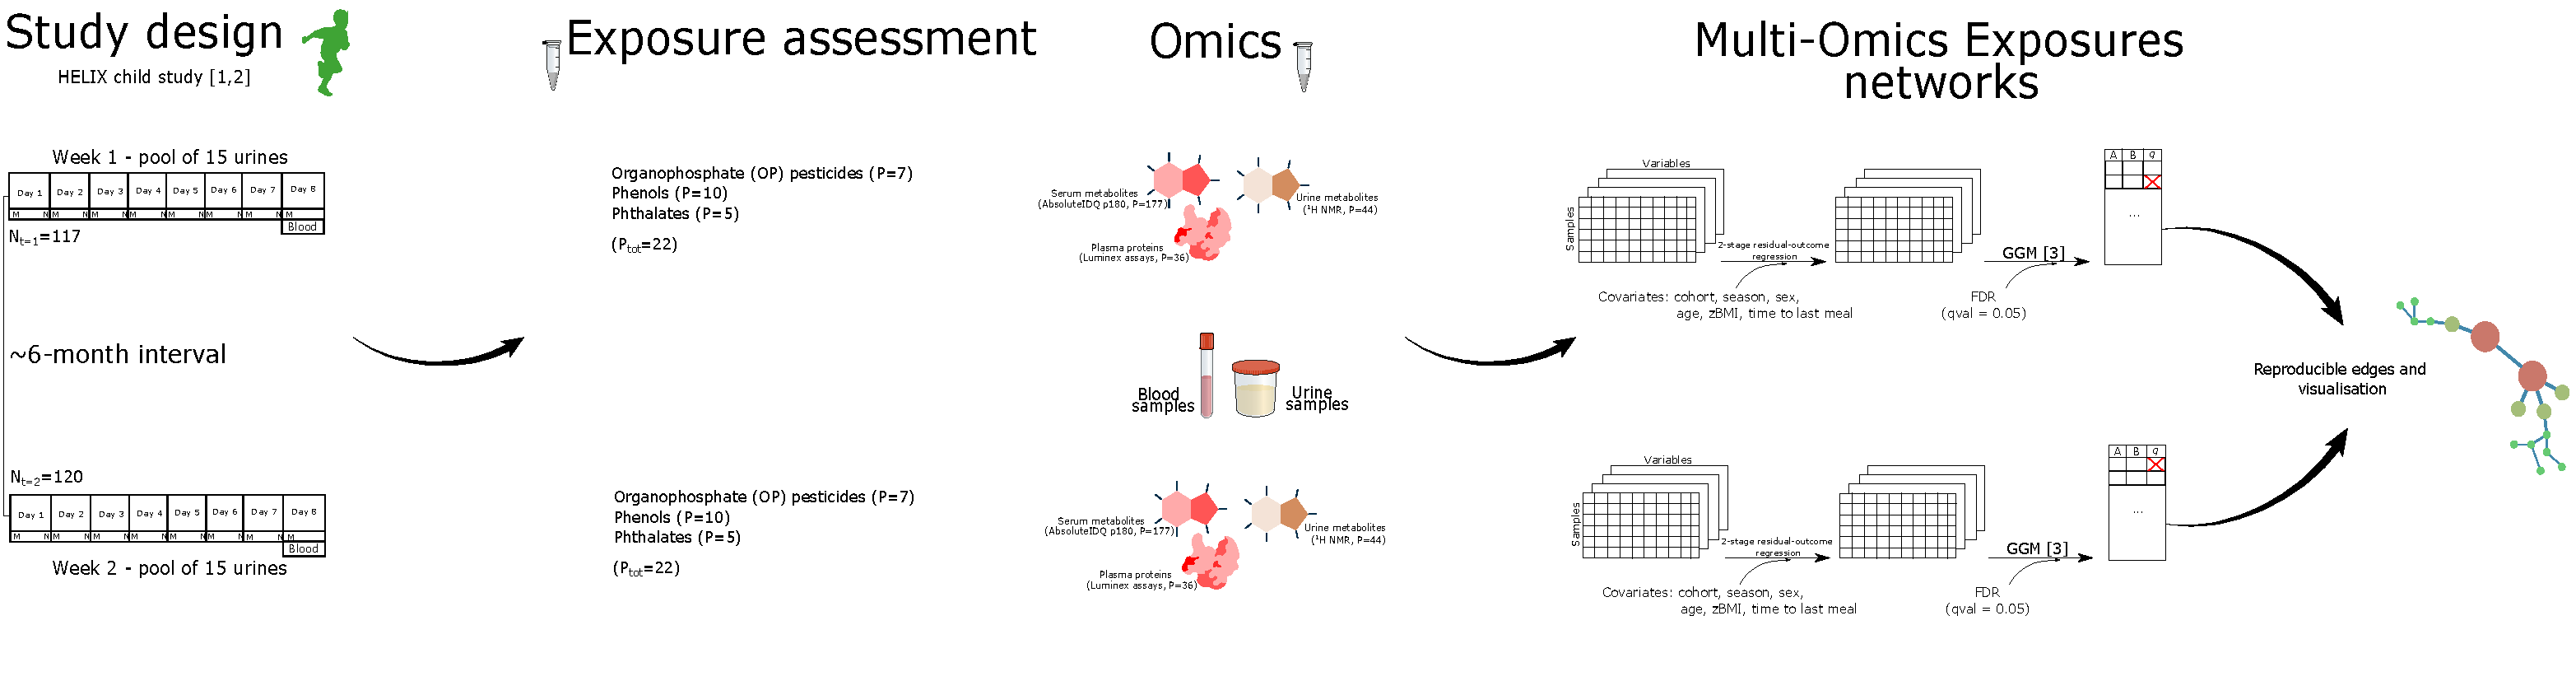
\includegraphics[height=19cm,width=75cm]{images/methods.pdf}
		%\includesvg{images/methods}
	\end{figure}
  \end{block}

\end{column}

\separatorcolumn
\end{columns}

%%%%%%%%%%%%%%%%%%%%%%%%%%%%%%%%%%%%%%%%%%%%%%%%%%%%%%%%%%%%%%%%%%%%%

\begin{columns}[t]
\separatorcolumn

\begin{column}{3\colwidth}

  \begin{block}{Results}
  \begin{columns}
  
	\begin{column}{0.2\textwidth}
		%\documentclass{article}

\usepackage{tabularx}

\begin{document}

\begin{table}[]
	\centering
	\begin{tabularx}{\linewidth}{lcc}
		\textbf{Characteristic} & $N_{t=1} = 117$\textsuperscript{1} & $N_{t=2} = 120$\textsuperscript{1} \\ 
		\hline
		\textbf{cohort} & & \\ 
		\enspace BIB & 27 (23\%) & 27 (22\%) \\ 
		\enspace KANC & 27 (23\%) & 26 (22\%) \\ 
		\enspace RHEA & 29 (25\%) & 29 (24\%) \\ 
		\enspace SAB & 34 (29\%) & 38 (32\%) \\ 
		\textbf{sex} &  \\ 
		\enspace female & 49 (42\%) & 50 (42\%) \\ 
		\enspace male & 68 (58\%) & 70 (58\%) \\ 
		\textbf{age} & 6.73 (6.38, 7.80) & 7.37 (6.89, 8.83) \\ 
		\textbf{ethnicity} &  \\ 
		\enspace Caucasian & 106 (91\%) & 109 (91\%) \\ 
		\enspace Pakistani & 10 (8.5\%) & 10 (8.3\%) \\ 
		\enspace Other & 1 (0.9\%) & 1 (0.8\%) \\ 
		\textbf{zBMI} & 0.36 (-0.23, 1.12) & 0.34 (-0.25, 1.17) \\ 
	\end{tabularx}
	\caption{Population description. \textsuperscript{1}n (\%); Median (IQR)}
\end{table}

\end{document}

		%\begin{table}[]
	\centering
	\begin{tabularx}{\linewidth}{llcccccc}
		Node A & Node B & $N$ & $P$\textsuperscript{1} & $N_{t=1}$ & $P_{t=1}$\textsuperscript{1} & $N_{t=2}$ & $P_{t=2}$\textsuperscript{1} \\ 
		\hline
		e & e & 20 & 9 & 48 & 5 & 50 & 5 \\ 
		e & ms & 1 & 0 & 44 & 4 & 71 & 6 \\ 
		e & mu & 5 & 2 & 59 & 6 & 67 & 6 \\ 
		ms & ms & 148 & 65 & 319 & 30 & 343 & 31 \\ 
		ms & mu & 7 & 3 & 168 & 16 & 184 & 17 \\ 
		ms & p & 2 & 1 & 86 & 8 & 82 & 7 \\ 
		mu & mu & 20 & 9 & 128 & 12 & 129 & 12 \\ 
		p & mu & 2 & 1 & 93 & 9 & 76 & 7 \\ 
		p & p & 24 & 10 & 84 & 8 & 77 & 7 \\ 
	\end{tabularx}
	\caption{Network description. \textsuperscript{1}$\%$}
	\label{table:edges}
\end{table}


		%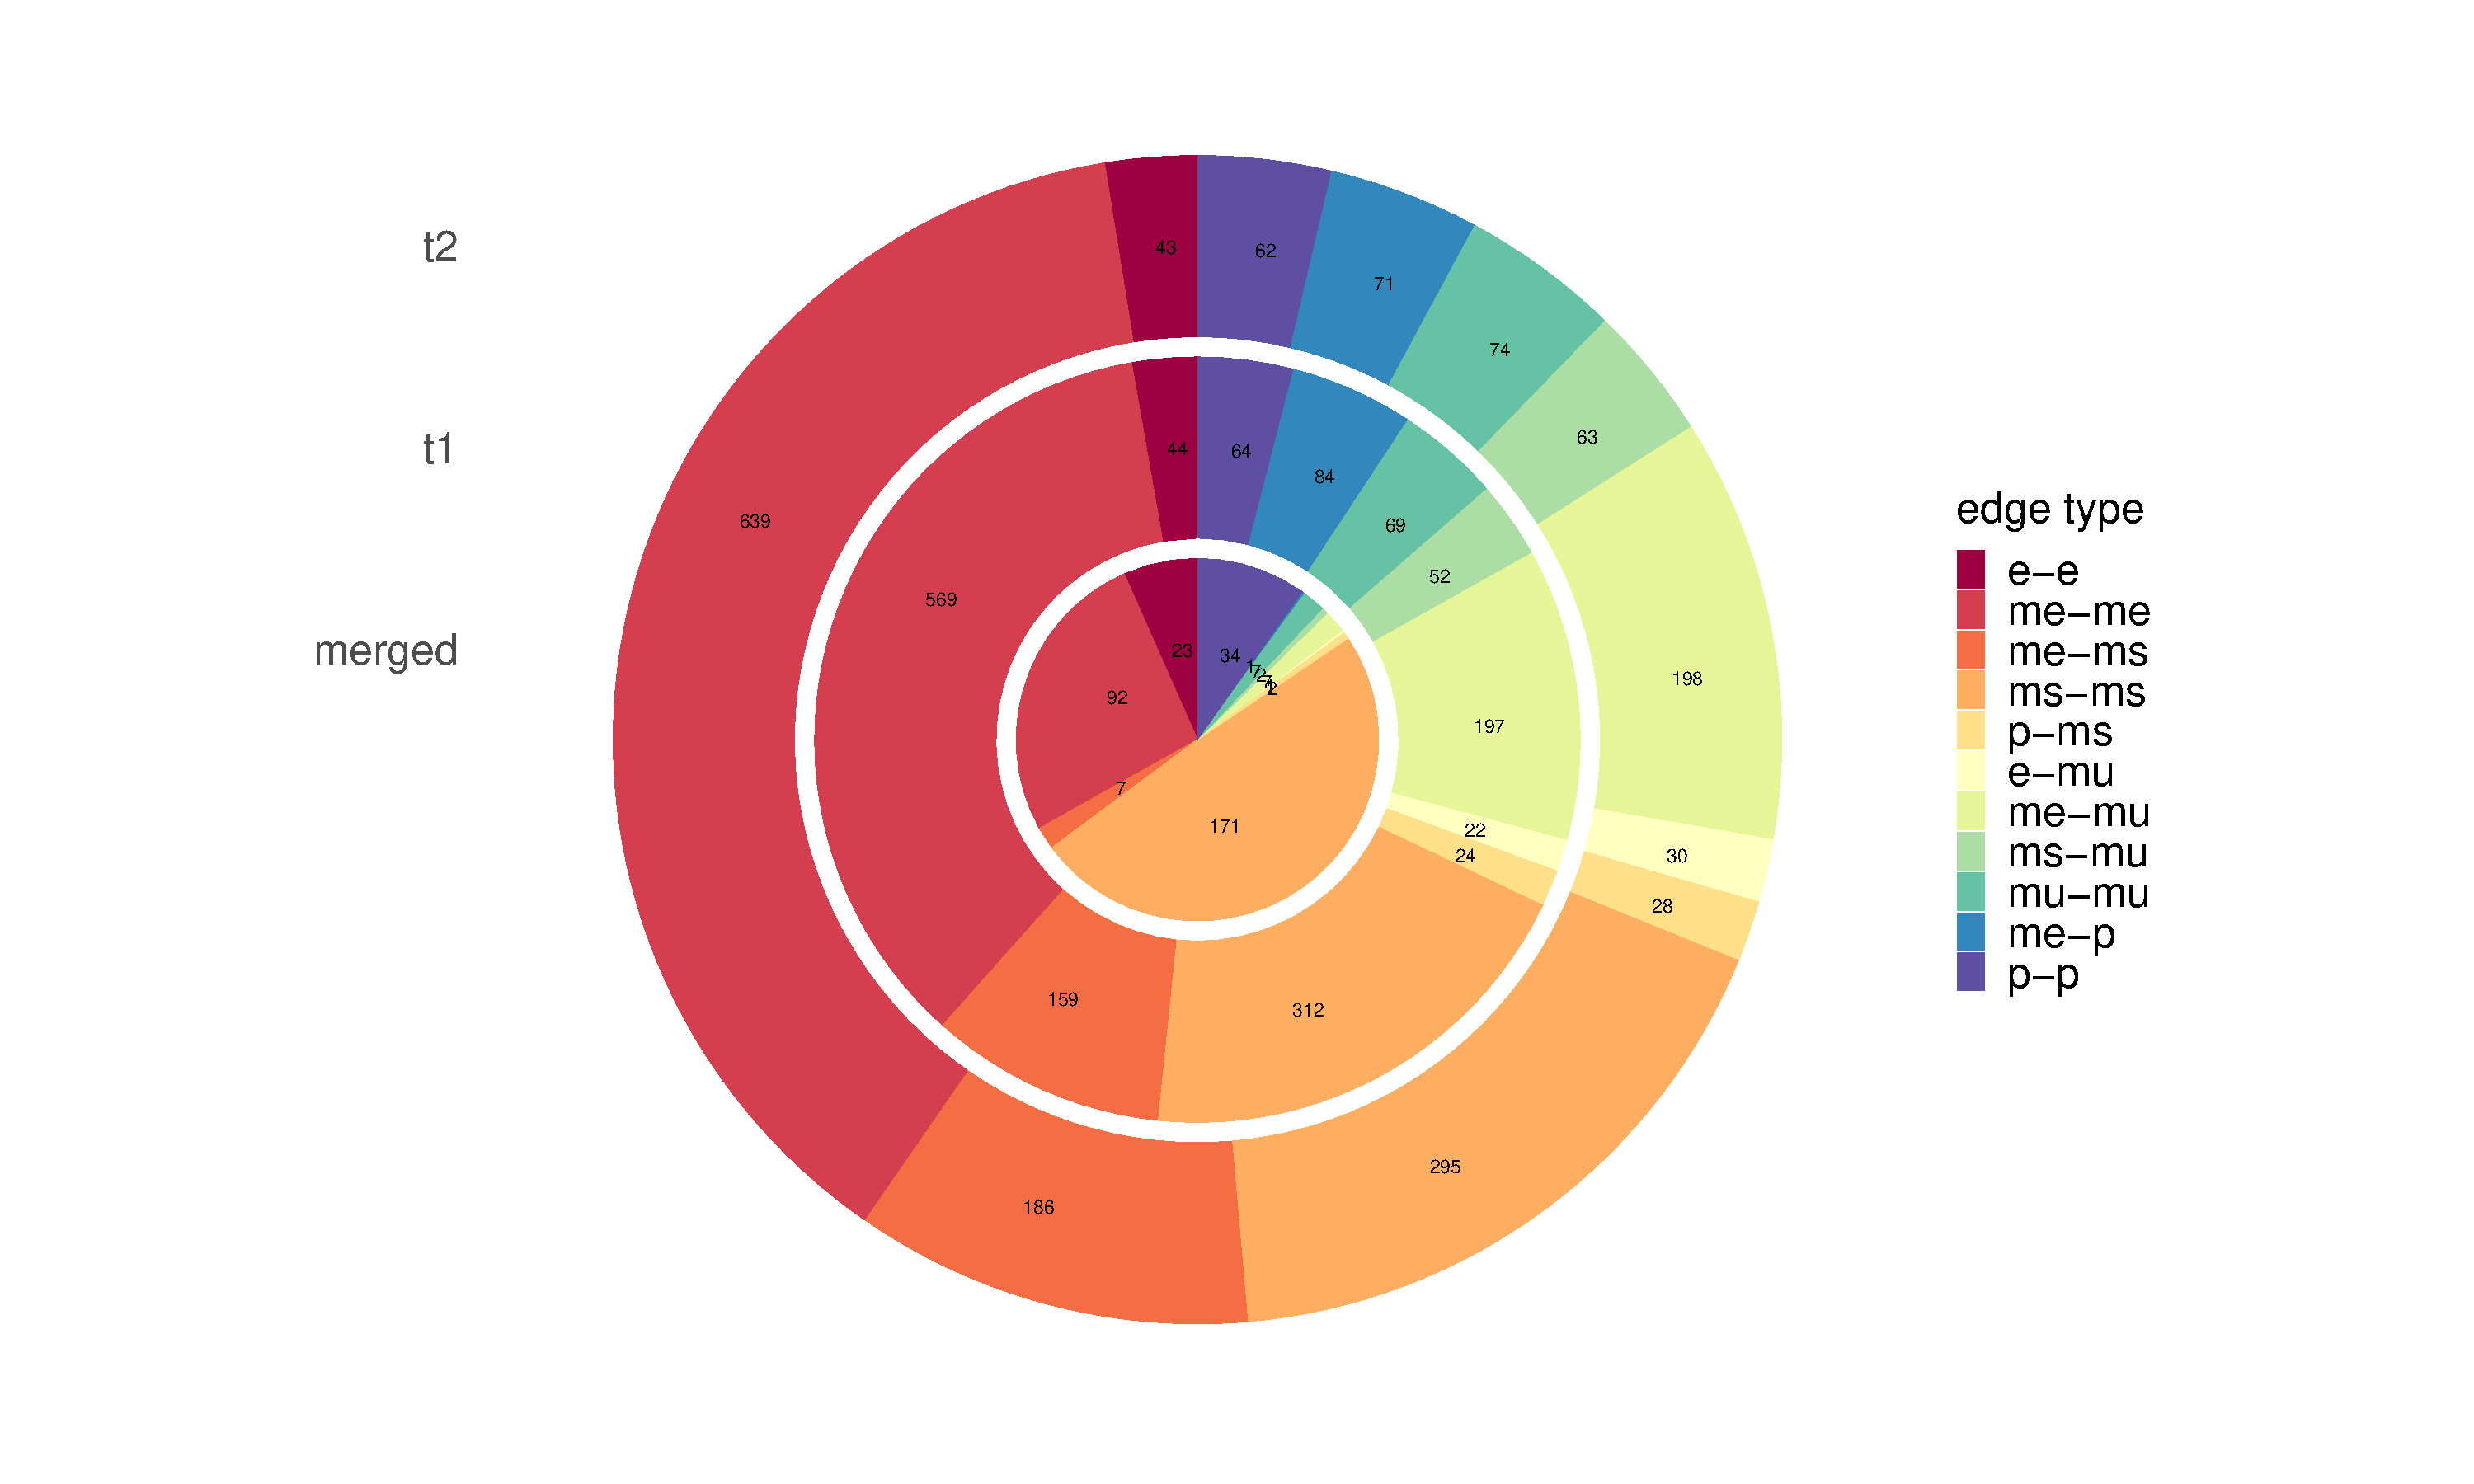
\includegraphics[width=\columnwidth]{images/piechart_edges}
		
		\begin{figure}
			\centering
			\subfloat[Merged network showing all the connected components.]{
				%\label{}
				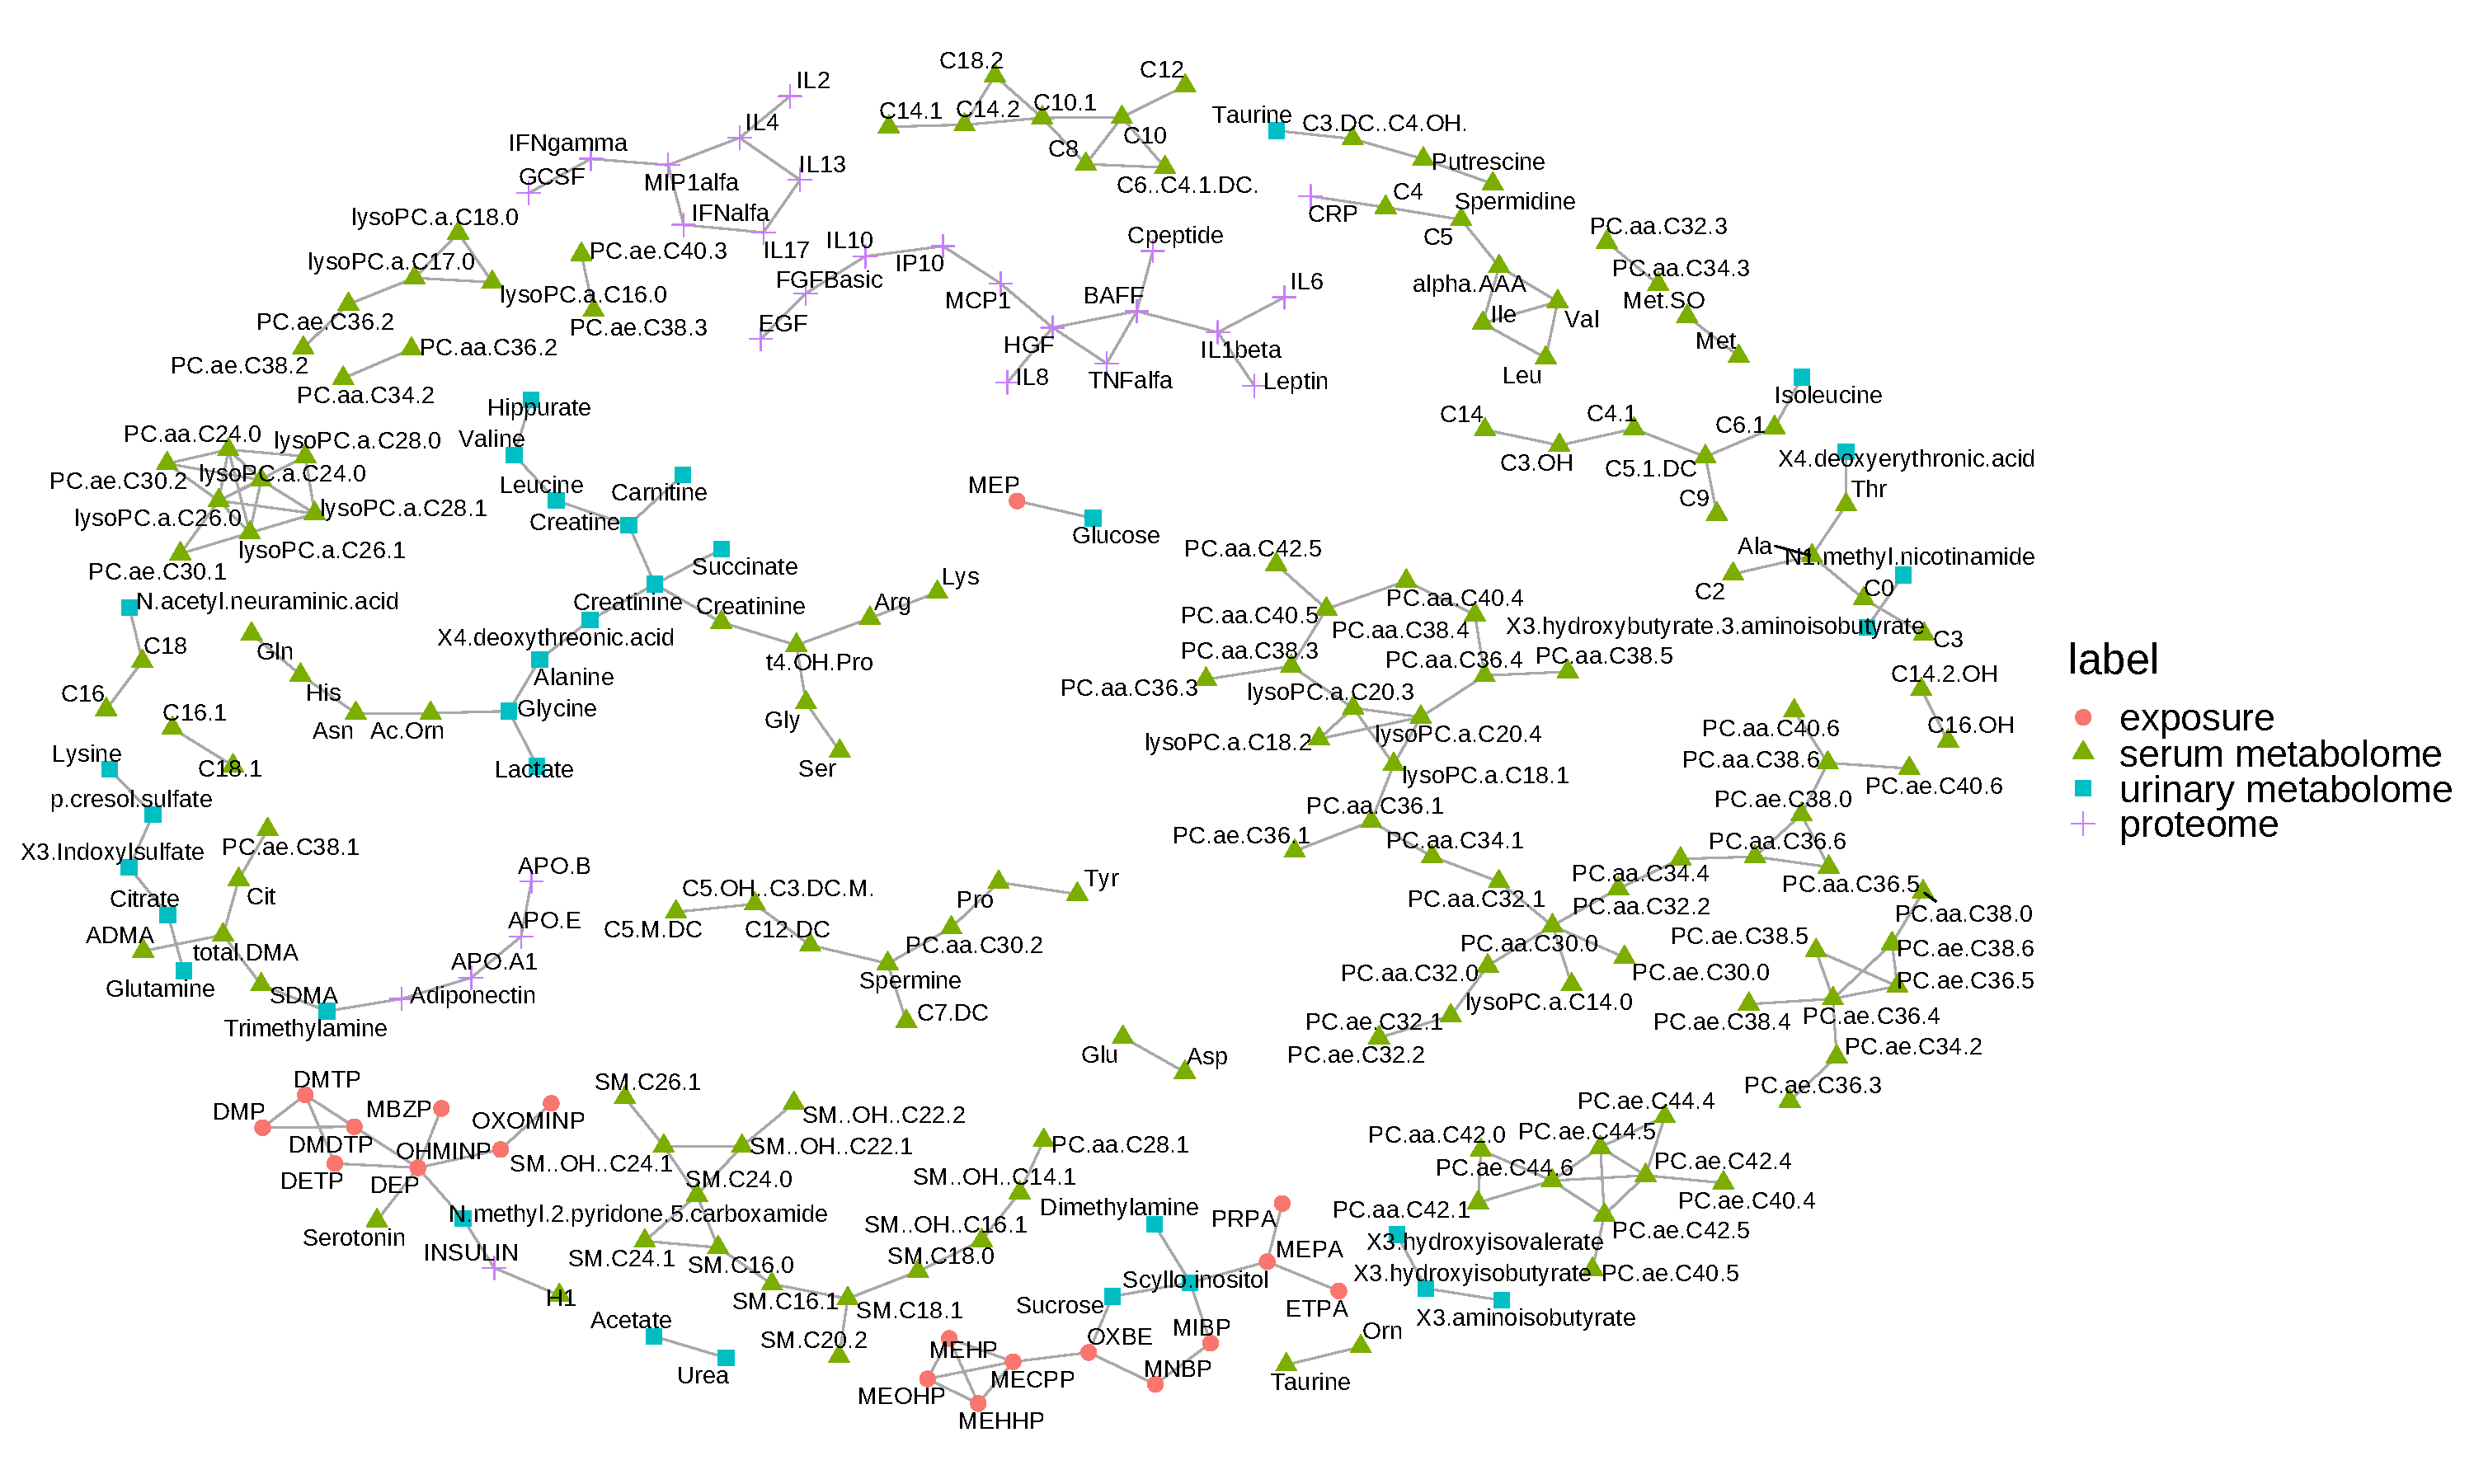
\includegraphics[width=\columnwidth]{../eurion22/images/merged_5}}\\
			\subfloat[Pie chart showing the proportion of edge types for the time-specific and merged networks. e = exposure, ms = serum metabolite, mu = urinary metabolite, p = protein.]{
				\label{figure:piechart}
				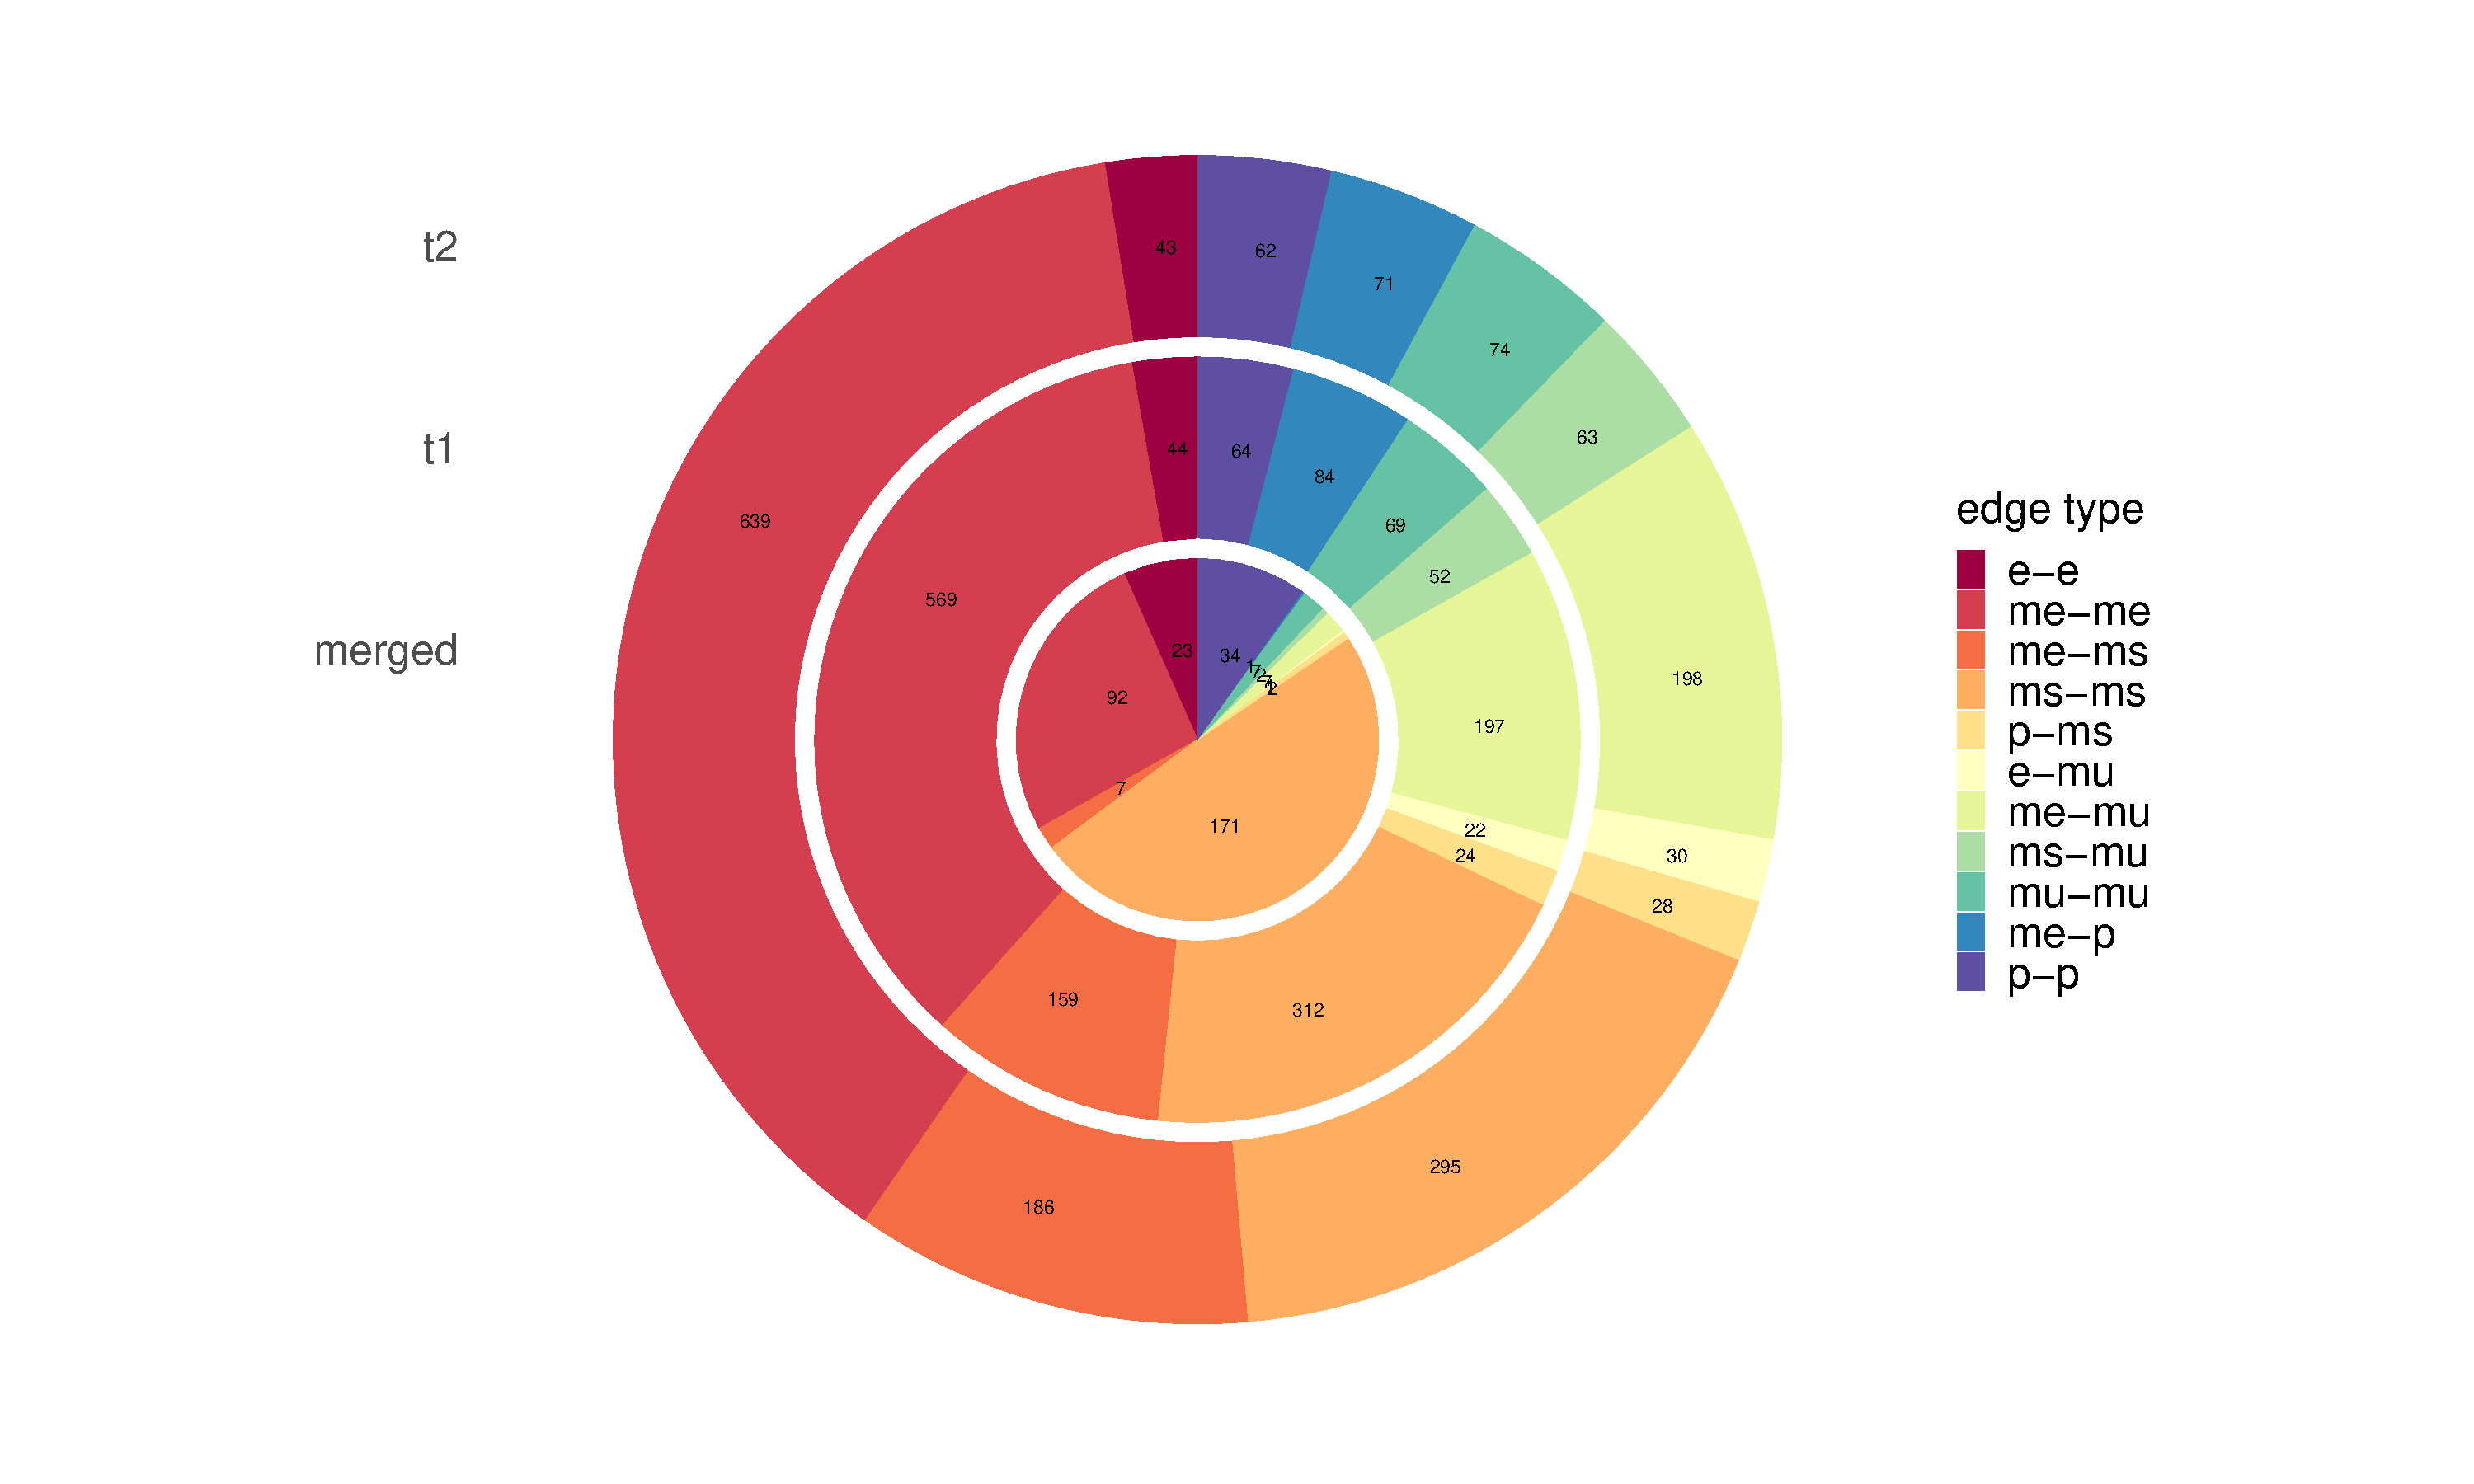
\includegraphics[width=\columnwidth]{images/piechart_edges}}
			\caption{Multi-Omics - EDCs association network.}
		\end{figure}				
		
	\end{column}
	
	\begin{column}{0.8\textwidth}
	
		\begin{itemize}
			\item The time-specific networks ($N_{\text{edges}}=1,064$, $N_{\text{edges}}=1,109$) included associations of comparable strength ($\rho = 0.09$ $(-0.09, 0.11)$ for both) and statistical significance ($\text{q} = 0.008$ $(0.001, 0.025)$, $\text{q} = 0.01$ $(0.001, 0.027)$). The significant edges represented less than $3\%$ of the possible connections
			\item The merged network consisted of $N_{\text{edges}}=229$
			\item Graph merging led to the exclusion of the majority of exposure-omic connections (Figure~\ref{figure:piechart}). Notably, none of the protein-exposure associations were reproducible
			\item The merged network consisted of $32$ connected components, $3$ of which included mixed exposure-omic connections (Figure~\ref{fig:ccs})
		\end{itemize}			
	
		\begin{figure}
				\centering
				\subfloat[]{
					%\label{}
					\includegraphics[width=.3\linewidth]{../eurion22/images/cc_4}}%
				\qquad
				\subfloat[]{
					%\label{}
					\includegraphics[width=.3\linewidth]{../eurion22/images/cc_6}}%
				\qquad
				\subfloat[]{
					%\label{}
					\includegraphics[width=.3\linewidth]{../eurion22/images/cc_23}}%
				\caption{Clusters (i.e., connected components) of EDC exposure-omic associations.}
				\label{fig:ccs}
		\end{figure}
		
		\begin{block}{Conclusions}
			\begin{itemize}
				\item We integrated Multi-Omic and exposure data from a child cohort using an integrative approach, and we identified associations reproducible across time points
				\item The association between DEP and Serotonin ($\rho=0.09$ for both time points) was reproducible. Exposure to Organophosphate pesticides has been linked to a variety of brain disorders [4], potentially through the serotonergic system
				\item In future work we plan to include methylation data
			\end{itemize}
		\end{block}
		
	\end{column}
  
  \end{columns}
  \end{block}

\end{column}

\separatorcolumn
\end{columns}
\end{frame}

\end{document}
